\chapter{Introduction au calcul littéral}\label{ChCalculLitteral}

\vspace{5cm}
\begin{acquis}
\begin{itemize}
\item 
\item 
\item 
\end{itemize}
\end{acquis}


\activites  
\begin{activite}[Supprimer des parenthèses]

\begin{partie}[Un signe « + » devant des parenthèses]
\begin{enumerate}
\item Complète : $4x + (3 -7x) =  4x + \left((+ ...) + (-...)\right)$.

Écris alors cette expression sans parenthèse puis rédige une règle pour ajouter une somme algébrique. Que peut-on dire de parenthèses précédées d'un signe + ?
\item Écris l'expression suivante sans parenthèse : $G = 5 + (-6x + 1)$.
\end{enumerate}
\end{partie}

\begin{partie}[Un signe « $-$ » devant des parenthèses]
\begin{enumerate}
\item Quel est l'opposé de 5 ? Et celui de $-6,5$ ? Que vaut la somme de deux nombres opposés ? Que peut-on dire de deux nombres dont la somme est égale à 0 ?
\item Complète :
    \subitem $-3 + ... = 0$ donc l'opposé de $-3$ est ... ;
    \subitem $-3x^2 + ... = 0$ donc l'opposé de $-3x^2$ est ... ;
    \subitem $... + 5 = 0$ donc l'opposé de 5 est ... ;
    \subitem $3 + x + ... = 0$ donc l'opposé de $3 + x$ est ... ;
    \subitem $-x + ... = 0$ donc l'opposé de $-x$ est ... ;
    \subitem $-2x + 1 + ... = 0$ donc l'opposé de $-2x + 1$ est ... ;
    \subitem $... + 2x = 0$ donc l'opposé de $2x$ est ... ;
    \subitem $2 -x^2 + ... = 0$ donc l'opposé de $2 -x^2$ est ... .
\item Rappel : $a-b = a + \text{ opposé de } b$.

Complète : $F = 2x -(3 + x) = 2x + (...)$.

Déduis-en l'expression de F sans parenthèse.

\item De la même façon, écris sans parenthèse $G = 4 -(2 -x^2)$ et $H = 2x + 3 -(-2x + 1)$.

Rédige une règle pour soustraire une somme algébrique.
\end{enumerate}       
\end{partie}

\end{activite}



\begin{activite}[Écrire une expression littérale]

Avec des petits carrés identiques, disposés comme le montrent les figures ci-dessous, on constitue un nouveau carré.

\begin{center}
    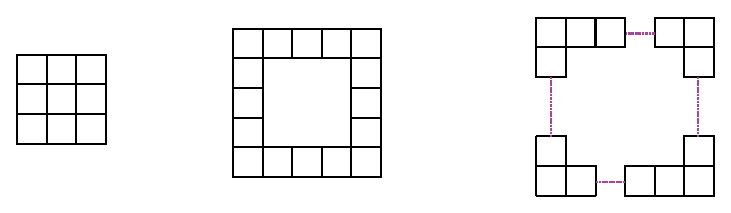
\includegraphics[width=.8\linewidth]{CLacti1}
\end{center}

\begin{enumerate}
\item Réalise une figure avec quatre petits carrés sur un côté. Indique le nombre total de carrés coloriés.

Recommence avec une figure de six petits carrés de côté.

S'il y a 100 petits carrés sur le côté, combien y-a-t-il de carrés coloriés au total ?
\item On appelle $n$ le nombre de petits carrés d'un côté. On veut obtenir une formule en fonction de n qui donne le nombre total de carrés coloriés dans le nouveau carré.
    \begin{enumerate}
        \item Chloé dit : « Je pense que la formule est $4n$ ! ».
        
        Sofiane lui répond alors : « Mais non ! Tu en as trop ! ».

        Justifie la réponse de Sofiane et établis une première formule.
        
        \item Sur les cahiers de trois élèves, on observe les schémas suivants :
        
        \begin{center}
        Schéma de Jean \hfill Schéma de Fatima \hfill Schéma de Bakari
            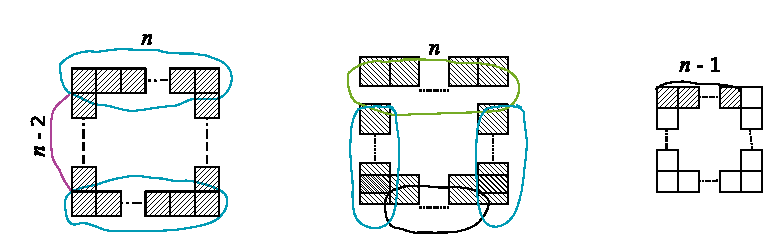
\includegraphics[width=.8\linewidth]{CLacti2}
        \end{center}

        En suivant les découpages de Jean et de Fatima, établis deux nouvelles formules.
        
        À l'aide de son schéma, Bakari remarque que le nombre de carrés coloriés est un multiple de 4.
        
        Justifie sa remarque et déduis-en une quatrième formule.
        
        \item En utilisant chacune de ces quatre formules, calcule le nombre total de carrés coloriés lorsqu'il y en a 15 sur un côté. Les résultats trouvés étaient-ils prévisibles ?
    \end{enumerate}
\end{enumerate}
\end{activite}



\begin{activite}[Conjecturer, démontrer]

On considère le programme de calculs suivant :

\begin{center}
    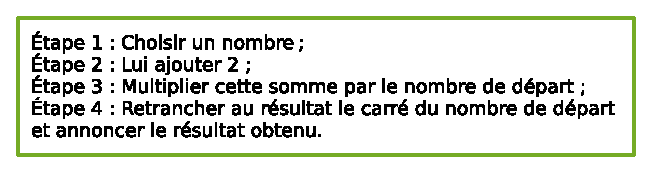
\includegraphics[width=.6\linewidth]{CLacti3}
\end{center}

\begin{enumerate}

\item Effectue le programme en choisissant 5 comme nombre de départ puis $-8$ et enfin $3,45$. Quelle remarque peux-tu faire ?
\item\label{CLact1} Dans un tableur, reproduis le tableau ci-dessous.

\begin{center}
    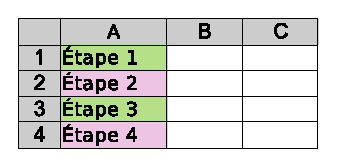
\includegraphics[width=.3\linewidth]{CLacti4}
\end{center}

Complète la première ligne avec les nombres entiers de 1 à 10 puis programme les cellules pour qu'elles affichent les résultats pour chaque étape du programme de calculs. Que remarques-tu ?
\item\label{CLact2} Remplace les nombres de la première ligne par des nombres entiers négatifs puis par des nombres décimaux relatifs. Que remarques-tu ?
\item On appelle $x$ le nombre de départ. Écris les étapes en fonction de $x$ et retrouve alors ce que tu as remarqué aux questions \ref{CLact1} et \ref{CLact2}.
\end{enumerate}
\end{activite}



\begin{activite}[L'art du contre-exemple]

\begin{enumerate}
\item Calcule $x^2 + 3$ puis $3x + 1$ en remplaçant d'abord $x$ par 1 puis par 2. Que remarques-tu ? Est-ce que  $x^2 + 3 = 3x + 1$ ? Justifie.
\item En étudiant un cube, Zoé remarque qu'il possède $F = 6$ faces et $S = 8$ sommets. Elle écrit $F + 2 = S$. Cette formule est-elle vraie pour un parallélépipède ? Est-elle vraie pour la pyramide ci-dessous ?

\begin{center}
    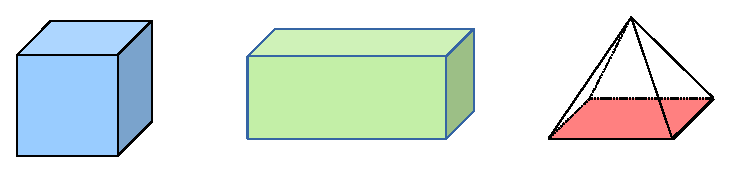
\includegraphics[width=.8\linewidth]{CLacti5}
\end{center}

\end{enumerate}
\end{activite}



\begin{activite}[Rectangles cousins]

\begin{enumerate}
\item Calcule le périmètre et l'aire des deux rectangles suivants. Que remarques-tu ?

\begin{center}
    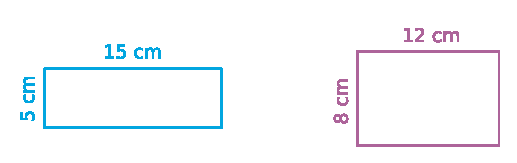
\includegraphics[width=.6\linewidth]{CLacti6}
\end{center}

Dans cette activité, on s'intéresse uniquement aux rectangles dont le périmètre est 40\,cm.

\item Un 3\up{e} rectangle a pour longueur $L = 16,5$\,cm. Calcule sa largeur $\ell$ puis son aire. 

\begin{center}
    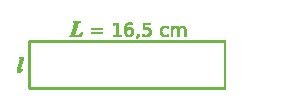
\includegraphics[width=.3\linewidth]{CLacti7}
\end{center}

\item Donne les mesures d'un 4\up{e} rectangle de même périmètre.
\item La longueur peut-elle valoir 8\,cm ? Et 21\,cm ? Justifie et donne les valeurs possibles pour la longueur.
\item Écris une expression qui permet de calculer la largeur $\ell$ en fonction de la longueur $L$. 
\item En voulant exprimer l'aire $\mathcal{A}$ du rectangle en fonction de sa longueur $L$, des élèves ont donné les réponses suivantes.
    \subitem Gaël	: $\mathcal{A} = L \times 20 - L$
	\subitem Inès	: $\mathcal{A} = 2 \times L + 2 \times (20 - L)$
	\subitem Hamid	: $\mathcal{A} = L \times (20 - L)$
	\subitem José	: $\mathcal{A} = L \times 20 - 2 \times L$
	\subitem Karen	: $\mathcal{A} = 20 L - L^2$
	\subitem Liam	: $\mathcal{A} = L^2 - 20 \times L$

Parmi ces expressions, lesquelles sont fausses ? Y a-t-il plusieurs bonnes réponses ? Justifie.

\item À l'aide d'un tableur, calcule l'aire de ces rectangles pour toutes les valeurs entières de $L$ possibles. 
\item Pour quelle valeur de $L$ l'aire semble-t-elle la plus grande ?
\end{enumerate}
\end{activite}

 



                                          




\cours
\section{Définitions}

\begin{definition}
\begin{itemize}
    \item Une expression littérale est une expression mathématique qui contient une ou plusieurs lettres.
    \item Pour tout nombre $a$, on peut écrire :
        \subitem $a \times a = a^2$	(qui se lit « $a$ au carré ») ;
		\subitem $a \times a \times a = a^3$ (qui se lit « $a$ au cube »).
	\item Un monôme est une expression de la forme $ax^n$ où $a$ est un nombre appelé coefficient du monôme et $n$ un nombre entier naturel appelé degré du monôme.
\end{itemize}
\end{definition} 

\begin{exemple*1}

$4a+1$ ; $2n^2$ ; $2ab-6$ ; $xy^2$ sont des expressions littérales

$x^2$ ; $5x^3$ ; $-12x$ ; $25x^2$ sont des monômes

$12ab$ ; $3xy$ ne sont pas des monômes
\end{exemple*1}


\begin{definition}
Un polynôme est une somme de monômes. Un polynôme avec deux termes est appelé binôme, avec trois termes, trinôme.
\end{definition} 

\begin{exemple*1}

$5x^3-3$ est un polynôme également appelé binôme

$3x^2+5x-7$ est un polynôme également appelé trinôme

$-5x^3+x^2-12x+23$ est un polynôme
\end{exemple*1}


\section{Simplification d'une expression littérale}
       
\begin{aconnaitre}
\begin{itemize}
    \item Il y a deux signes pour la multiplication : on peut utiliser indifféremment $\times$ et $\cdot$.
    \item \textbf{Pour simplifier l'écriture d'une expression littérale}, on peut supprimer le signe de multiplication devant une lettre ou une parenthèse.
\end{itemize}
\end{aconnaitre} 

\begin{remarque}
On ne peut pas supprimer le signe $\times$ entre deux nombres.
\end{remarque}

\begin{exemple*1}
Simplifie l'expression suivante : $A = -5 \times x + 7 \times (-4) \times (3 \times x -2)$.

\correction

\begin{tabular}{lcl}
$A = -5 \times x + 7 \times (-4) \times (3 \times x -2)$ & $\longrightarrow$ & On repère tous les signes $\times$. \\
$A = -5x + 7 \times (-4)(3x -2)$ & $\longrightarrow$ & On supprime les signes $\times$ placés devant une lettre \\
& &  ou une parenthèse. \\
$A = -5x -28(3x -2)$ & $\longrightarrow$ & On calcule si possible. \\
\end{tabular}

\end{exemple*1} 


\begin{methode*1}[Remplacer des lettres par des nombres]
Pour \textbf{calculer une expression littérale pour une certaine valeur des lettres}, il suffit de remplacer les lettres par ces valeurs. 
\exercice

Calcule l'expression $A = 5x(x + 2)$ pour $x = 3$.

\correction

\begin{tabular}{lcl}
$A = 5 \times x \times (x + 2)$ & $\longrightarrow$ & On replace les signes $\times$ dans l'expression $A$. \\
$A = 5 \times 3 \times (3 + 2)$ & $\longrightarrow$ & On remplace la lettre $x$ par sa valeur 3. \\
$A = 15 \times 5$ & $\longrightarrow$ & On effectue les calculs. \\
$A = 75$ & & \\
\end{tabular}

\end{methode*1}






\exercicesbase
\begin{colonne*exercice}
\serie{Utiliser une expression littérale}


\begin{exercice}[En électricité]
Une formule relie la Puissance $P$ consommée par un dipôle à la tension $U$ à ses bornes et à l'intensité $I$ qui le traverse :

$P = U \times I$ où $P$ s'exprime en Watts (W), $U$ en Volts (V) et $I$ en Ampères (A).

\begin{colenumerate}{1} 
\item Quelle puissance génère un courant de 220 V et d'intensité 3 A ?
\item Construis un tableau donnant toutes les puissances générées par un courant de 220 V pour des intensités entières allant de 1 A à 10 A. Que peut-on dire d'un tel tableau ?
\end{colenumerate} 
\end{exercice}

\begin{exercice}[Sur Internet et avec tableur !]

\begin{colenumerate}{1} 
\item S'il est 10 h à Paris en été, quelle heure est-il au même moment à New-York ? Moscou ? Tokyo ?
\item Paris est à l'heure d'été. À l'aide d'un tableur, programme une feuille de calcul qui donne l'heure qu'il est dans une dizaine de villes du monde quand on entre l'heure de Paris. 
\end{colenumerate} 
\end{exercice}



\begin{exercice}[Formule d'Euler -Poincaré]

Pour certains solides convexes (par exemple le cube), il existe une formule qui relie le nombre de sommets du solide ($S$), son nombre d'arêtes ($A$) et son nombre de faces ($F$) :
\[ S - A + F = 2 \].

\begin{colenumerate}{1} 
\item Vérifie que cette formule fonctionne bien avec un cube.
\item Si on connaît $A$ et $F$, peut-on trouver directement $S$ ? Écris une formule permettant de trouver $S$.
\item Combien d'arêtes a un solide convexe qui a 4 sommets et 4 faces ? Dessine-le à main levée.
\end{colenumerate} 
 
\end{exercice}




\begin{exercice}
Traduis les phrases suivante par une expression algébrique :

\begin{colenumerate}{1} 
\item Le produit de la somme de $x$ et de 3 par 6,
\item La différence de $x$ et du produit de 5 par $y$,
\item La somme du produit de $x$ par 3 et de la différence de $2x$ et de 5,
\item Le produit de la différence du carré de $x$ et de 7 par la somme de $x$ et de 12.
\end{colenumerate} 
 
\end{exercice}




\serie{Simplifier une expression littérale}




\begin{exercice}
Recopie les expressions en supprimant les signes $\times$ s'ils sont inutiles.
\begin{colenumerate}{2}
\item $A = 9 \times n$
\item $B = x \times 3$
\item $C = 12 \times (7 - 3)$
\item $D = 4 \times (3,2 + 6)$
\item $E = n \times x$
\item $F = 2 \times \pi \times R$
\item $G = (3 + 6) \times (7 - 1)$
\item $H = 16 \times 3,5$
\end{colenumerate}
\end{exercice}




\begin{exercice}
Recopie les expressions en ajoutant les signes $\times$ lorsqu'ils sont sous-entendus.

\begin{colenumerate}{2}
\item $A = 3x + 2$
\item $B = ab - 4$
\item $C = 5(2x - 7)$
\item $D = 2a(2 + 8)$
\item $E = 3a - 5b$
\item $F = ab + 3 \times 7a$
\item $G = b - a + 7(3x + 7)$
\item $H = a + a - 7b + 1$
\end{colenumerate}
\end{exercice}



\begin{exercice}

Écris le plus simplement possible.
\begin{colenumerate}{2}
\item $A = 3 \times a \times b$
\item $B = 3 \times a  + 3 \times b$
\item $C = 8 \times a \times 2$
\item $D = 5 + 3 \times b$ 
\item $E = 5 \times a + 3 + 2$
\item $F = 2 \times 3 \times a \times (b \times c)$
\end{colenumerate}
\end{exercice}

\begin{exercice}[]Écris le plus simplement possible.
\begin{colenumerate}{2}
\item $A = 7 \times a \times b \times 3$
\item $B = 7 + a \times b + 3$
\item $C = 3 \times (2 \times a + b) \times 5$
\item $D = (2,5 - 1) \times a \times b$
\end{colenumerate}
\end{exercice}

\begin{exercice}[]Simplifie les expressions en utilisant les notations "au carré" et "au cube".
\begin{colenumerate}{2}
\item $A = a \times a$
\item $B = b \times b \times b$
\item $C = c \times c \times 3$
\item $D = 9 + d  \times d \times d$
\item Aire d'un carré de côté $c$ : $c \times c = ...$
\item Aire d'un disque de rayon $r$ : $\pi \times r \times r = ...$
\end{colenumerate}
\end{exercice}

\begin{exercice}
Écris les expressions suivantes le plus simplement possible en utilisant les notations \og au carré\fg et \og au cube \fg si nécessaire.
\begin{colenumerate}{2}
\item $A = 1 \times a + a \times a$
\item $B = a \times a \times a - 0 \times b$
\item $C = 6 \times a \times a - a$
\item $D = 2 \times a \times 3 \times a$
\item $E = a \times a \times b \times 3$
\item $F = 1 \times a \times a \times b \times 0$
\item $G = a \times 2 \times b \times a \times b$
\item $H = (a + b)(a + b)$
\end{colenumerate}
\end{exercice}

\begin{exercice}
Écris les multiplications cachées.
\begin{colenumerate}{2}
\item $A = 5a^2$
\item $B = 2 - b^3$
\item $C = a^2 + 2b^3$
\item $D = a^2b^3$
\end{colenumerate}
\end{exercice}

\begin{exercice}[]
Si $x$ représente un nombre, comment écrire les expressions suivantes ?

\begin{colenumerate}{1} 
\item Le double de $x$.
\item Le tiers de $x$.
\item La somme de $x$ et de 13. 
\item La différence de $x$ et de 7. 
\item Le triple de la somme de 2 et de $x$.
\item Le tiers de la différence de 16 et $x$.
\end{colenumerate} 
\end{exercice}

\begin{exercice}[] Traduis par une phrase les expressions.
\begin{colenumerate}{2}
\item $A = x + 7$
\item $B = 3x$
\item $C = 2x + 1$
\item $D = 5 - 2x$
\item $E = (3 + x)(3 - x)$
\item $F = x2 + 5$
\end{colenumerate}
\end{exercice}

\begin{exercice}[] Calcule chaque expression pour la valeur de x indiquée.
\begin{colenumerate}{2}
\item $A = x^2$	pour $x = 2,5$
\item $B = 5x^2$	pour $x = 2$
\item $C = 4 + 2x^2$	pour $x = 0$
\item $D = x^3$	pour $x = 3$
\item $E = 2x^3$	pour $x = 5$
\item $F = 15 - x^3$	pour $x = 1$
\end{colenumerate}
\end{exercice}

\begin{exercice}
Calcule chacune des expressions suivantes pour $x = 3$ et $y = 2$.
\begin{colenumerate}{2}
\item $A = xy + 4$
\item $B = x - y + 8$
\item $C = xy - x - y + 4$
\item $D = xyx$
\end{colenumerate}
\end{exercice}

\begin{exercice}
Calcule chacune des expressions suivantes pour $x = 1$ et $y = 2$.
\begin{colenumerate}{2}
\item $A = x^2 + x + y$
\item $B = x^2 + 2xy + y^2$
\item $C = x^2y$
\item $D = x^2 + y^2$
\end{colenumerate}
\end{exercice}





\serie{Produire une expression littérale}





\begin{exercice}[Rectangles imbriqués]

\begin{center}
    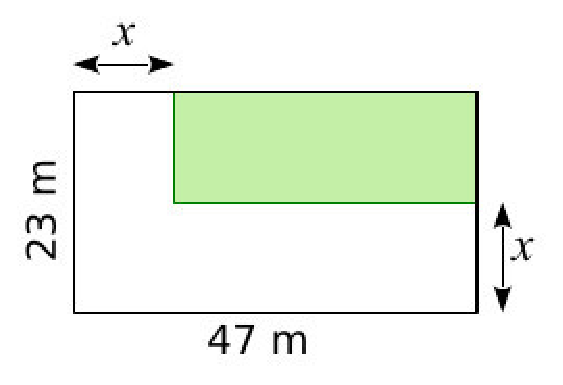
\includegraphics[width=.4\linewidth]{rectangle}
\end{center}

\begin{colenumerate}{1} 
\item Calcule l'aire de la partie coloriée en fonction de $x$.
\item Combien vaut cette aire si $x = 14,7$ m ?
\end{colenumerate} 
\end{exercice}

\begin{exercice}
Sachant que le quadrilatère $MATH$ est un parallélogramme, exprime tous les angles de la figure ci-dessous en fonction de $x$.

\begin{center}
    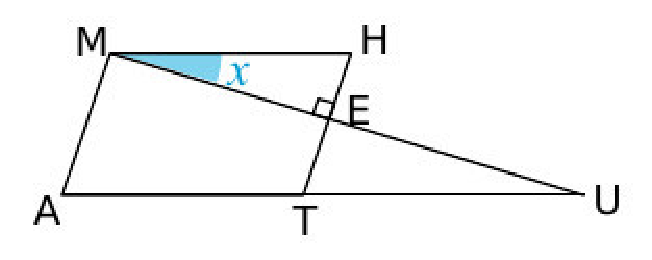
\includegraphics[width=.6\linewidth]{parallelogramme}
\end{center}


\end{exercice}


\begin{exercice}
Pour son téléphone portable, Grégoire paye : 12 € d'abonnement, $a$ € par SMS envoyé et 40 centimes d'euros par minute de communication. 

\begin{colenumerate}{1} 
\item Écris une expression permettant de calculer sa dépense sachant que ce mois-ci, Grégoire a envoyé 30 SMS et a utilisé $m $minutes de communication.
\item Quelle est cette dépense si $a = 0,8$ et $m = 150$ ?
\end{colenumerate} 
\end{exercice}



\begin{exercice}
Sandrine a construit un triangle tel que la longueur du petit côté vaut la moitié de celle du grand et la longueur du moyen vaut les trois quarts de celle du grand.

\begin{colenumerate}{1} 
\item Écris une expression permettant de calculer le périmètre du triangle en fonction de la longueur $L$ du plus grand des côtés.
\item Détermine le périmètre si $L$ vaut 7 cm.
\end{colenumerate} 
\end{exercice}



\begin{exercice}
Marc a rentré trois nombres en mémoire dans sa machine à calculer. Pour cela, il a utilisé les lettres $a$, $b$ et $c$. Il veut maintenant calculer les expressions suivantes :

$S = 2a - 3b + 7c + 5$

$T = 7a \times b + 4c - 8$

Calcule ces expressions pour $a = 12$, $b = 5$ et $c = 7$. Vérifie tes résultats à la calculatrice.
\end{exercice}



\serie{Supprimer les parenthèses}



\begin{exercice}
Replace dans chacune des expressions tous les signes $\times$ sous‑entendus.
\begin{colenumerate}{1}
\item $A = 3x^2 + 5x -10$
\item $B = 4y(21 -3y)$
\item $C = (2z -1)(5 -z)$
\end{colenumerate}
\end{exercice}

\begin{exercice}
Relie les expressions qui sont égales puis trouve l'intruse :

\begin{center}
    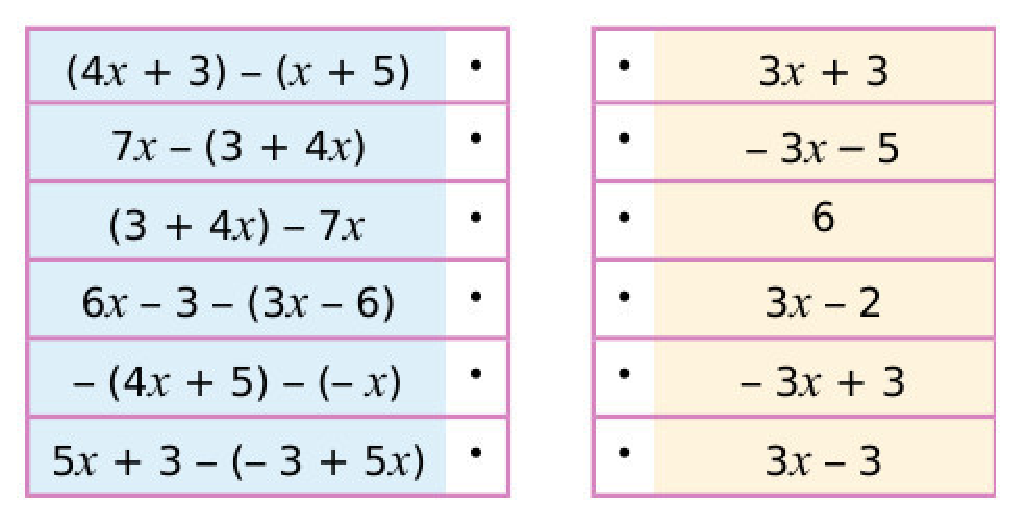
\includegraphics[width=.8\linewidth]{tableau1}
\end{center}
\end{exercice}



\begin{exercice}
Supprime les parenthèses puis réduis les expressions suivantes :
\begin{colenumerate}{1}
\item $A = 3x + \dfrac{1}{4} - (3-2x)$
\item $B =-(\dfrac{1}{3}x + 2) + (5x-3)$ 
\item $C =(\dfrac{2}{3}x + \dfrac{1}{3}) - (\dfrac{5}{6}+\dfrac{2}{6}x)$
\item $D = \dfrac{1}{2} + 2x -(x-\dfrac{3}{2})$
\end{colenumerate}
\end{exercice}


\begin{exercice}
Complète les développements.
\begin{colenumerate}{1}
\item $A = x(3 + 2x) = x \times .. + .. \times 2x = ... + ...$
\item $B = 3a(4b -...) = ... -15^2$
\item $C = 5x(3y -...) = ... xy -20x$
\end{colenumerate}
\end{exercice}




\serie{Substitution}




\begin{exercice}[] Calcule chaque expression pour la valeur de $x$ indiquée.
\begin{colenumerate}{2}
\item $A = x + 11$	pour $x = 7$
\item $B = 5x$	pour $x = 2$
\item $C = 14 + x$	pour $x = 3$
\item $D = 14x$	pour $x = 1,5$
\item $E = 2 + 2x$	pour $x = 5$
\item $F = 15 - 3x$	pour $x = 1$
\end{colenumerate}
\end{exercice}

\begin{exercice}
Teste chacune des égalités suivantes pour $x = 2$ puis pour $x = 3$.

\begin{colenumerate}{2} 
\item $4x - 10 = 8$
\item $4x - 12 = 0$
\item $2x - 4 = 5x - 10$
\item $3x - 7 = x + 1$
\end{colenumerate} 
\end{exercice}



\begin{exercice}
Teste chacune des égalités pour $x = 5$.

\begin{colenumerate}{2} 
\item $x^2 - 25 = 0$
\item $x^2 - 5 = 4x$
\item $x^2 = 10$
\item $3x - 7 = x2 + 1$
\end{colenumerate} 
\end{exercice}


\begin{exercice}
Dans chacun des cas proposés, détermine si l'égalité $3x + 5 = 2y - 4$ est vraie ou pas.

\begin{colenumerate}{2} 
\item $x = 1$ et $y = 1$
\item $x = 3$ et $y = 9$
\item $x = \dfrac{1}{3}$ et $y = 6$
\item $x = 1,5$ et $y = 1$
\item $x = 0$ et $y = 0$
\item $x = \dfrac{5}{3}$ et $y = 2$
\end{colenumerate} 
\end{exercice}

\begin{exercice}
À l'achat d'un portable, on propose deux forfaits possibles :
\begin{itemize}
\item Première offre : 0,25 € par SMS. 
\item Deuxième offre : abonnement de 2 € et 0,15 € par SMS.
\end{itemize}

On note $n $le nombre de SMS envoyés.

\begin{colenumerate}{1} 
\item Pour chaque offre, écris le coût du forfait en fonction de $n$. 
\item Estelle a payé 4,70 € pour 18 SMS envoyés. Quel forfait a-t-elle choisi ?
\end{colenumerate} 
\end{exercice}



\begin{exercice}
Recopie puis complète l'arbre de calcul.
\begin{center}
    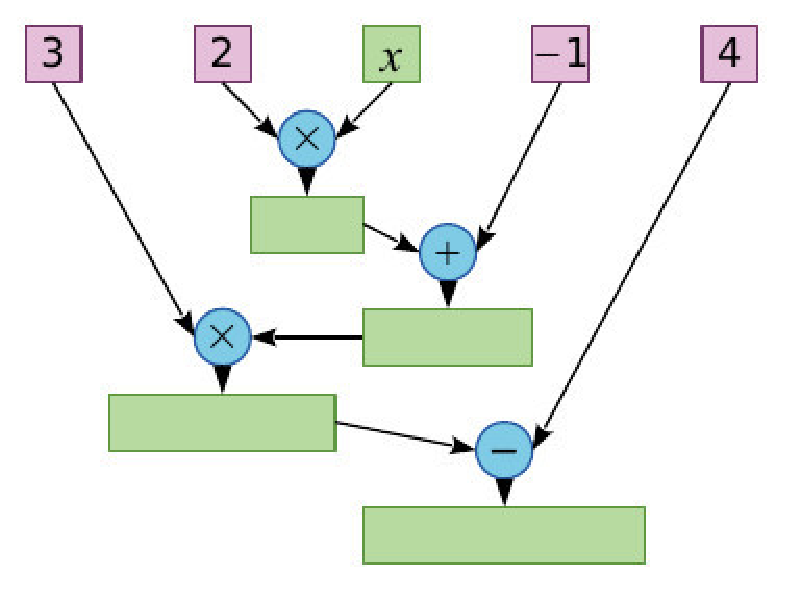
\includegraphics[width=.6\linewidth]{arbre1}
\end{center}
\end{exercice}


\begin{exercice}[À l'envers !]

\begin{colenumerate}{1} 
\item En t'inspirant de l'exercice précédent, crée un arbre de calcul pour obtenir l'expression : $5(4 - 3x) + 7$.
\item Calcule l'expression pour $x = 0$ puis $x =\dfrac{1}{2}$.
\end{colenumerate} 
\end{exercice}


\begin{exercice}[Comparaison de périmètres]
Exprime en fonction de $x$ et $y$ les périmètres du carré et du rectangle suivants.

\begin{center}
    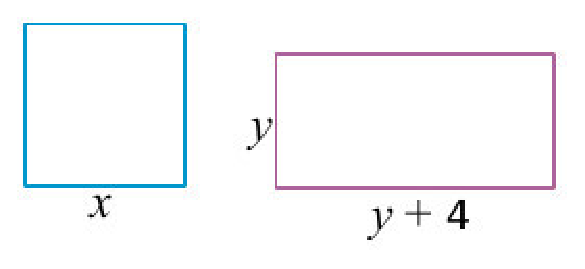
\includegraphics[width=.5\linewidth]{carreRect}
\end{center}

Pour les valeurs de $x$ et de $y$ suivantes, le périmètre du carré est-il supérieur à celui du rectangle ?

\begin{colenumerate}{1} 
\item $x = 2$ et $y = 1$
\item $x = 3$ et $y = 1$
\item $x = 6$ et $y = 3$
\item $x = 10$ et $y = 7$
\end{colenumerate} 
\end{exercice}


\begin{exercice}[Une suite de nombres]

Voici une liste de 6 nombres :

2 ; 5 ; 7 ; 12 ; 19 ; 31.

Pour obtenir cette liste, on a choisi les deux premiers nombres au hasard (2 et 5). Les nombres suivants sont obtenus en ajoutant les deux qui précèdent. 

On note $S$ la somme de ces 6 nombres.

\begin{colenumerate}{1} 
\item Vérifie que cette somme $S$ est égale à 4 fois le cinquième nombre de la liste.
\item Avec un tableur, vérifie-le en choisissant d'autres nombres de départ.
\item Prouve que cette affirmation est toujours vraie, quels que soient les nombres choisis.
\end{colenumerate} 
\end{exercice}

\begin{exercice}
Vanessa a acheté un cahier à 2 € et trois classeurs.

\begin{colenumerate}{1} 
\item Exprime le prix total qu'elle a payé en fonction du prix en euros (noté $x$) d'un classeur.
\item Elle a payé 23 € en tout. Utilise un tableur pour retrouver le prix d'un classeur.
\end{colenumerate} 
\end{exercice}


\begin{exercice}
Recopie les expressions suivantes en rajoutant les signes $\times$ sous-entendus puis calcule-les pour $x = 2$ :

\begin{colenumerate}{2} 
\item $A = 2x$
\item $B = 4x +5$
\item $C = 4(x -3)(x + 8)$
\item $D = 3x -2(5x -15)$
\item $E = 9x^2$
\item $F = 7 -2x$
\item $G = 2(3x -2)$
\item $H = x(x + 2) -4x$
\item $I = 4x^2 -2x(4 -x)$
\item $J = -3x^2 + 5x -4$
\end{colenumerate}
\end{exercice}

\begin{exercice}[] Recopie et complète le tableau suivant :

\renewcommand*\tabularxcolumn[1]{>{\centering\arraybackslash}m{#1}}
\renewcommand{\arraystretch}{1.6}
\begin{cltableau}{\linewidth}{4}
\hline
 & $x = 4$ & $x = 0$ & $x = -2$ \\ \hline
$3(2x -7) -5x$ & & & \\ \hline
$(x -4)(x -2)$ & & & \\ \hline
$(2 -x)^2$ & & & \\ \hline
\end{cltableau}
\end{exercice}

\begin{exercice}
Calcule les expressions suivantes :
\begin{colenumerate}{1} 
\item $A = 3t^2 + 6t -8$ pour $t = 3$ ;
\item $B = 5x^2 -3x + 7$ pour $x = -2$ ;
\item $C = -3y^2 -5y -8$ pour $y = -3$.
\end{colenumerate}
\end{exercice}




\serie{Programme de calculs}



\begin{exercice}
Exprime en fonction de $x$ les expressions suivantes ($x$ étant non nul) :

\begin{colenumerate}{1} 
\item l'opposé de $x$ ;
\item l'inverse de $x$ ;	
\item l'opposé du carré de $x$;
\item le carré de l'opposé de $x$ ;	
\item l'opposé de l'inverse de $x$ ;
\item le carré de l'inverse de $x$.
\end{colenumerate} 
\end{exercice}

\begin{exercice}
Si on note $z$ l'âge en années d'Alexis aujourd'hui, comment note-t-on :

\begin{colenumerate}{1} 
\item l'âge qu'il aura dans deux ans ?
\item le double de son âge ?
\item le triple de l'âge qu'il avait il y a quatre ans ?
\item la moitié de l'âge qu'il aura dans cinq ans ?
\item son année de naissance ?
\end{colenumerate} 
\end{exercice}

\begin{exercice}
Relie chaque phrase de la première colonne avec l'expression qui lui correspond où $y$ est le prix d'achat de l'article en euros :
\begin{center}
    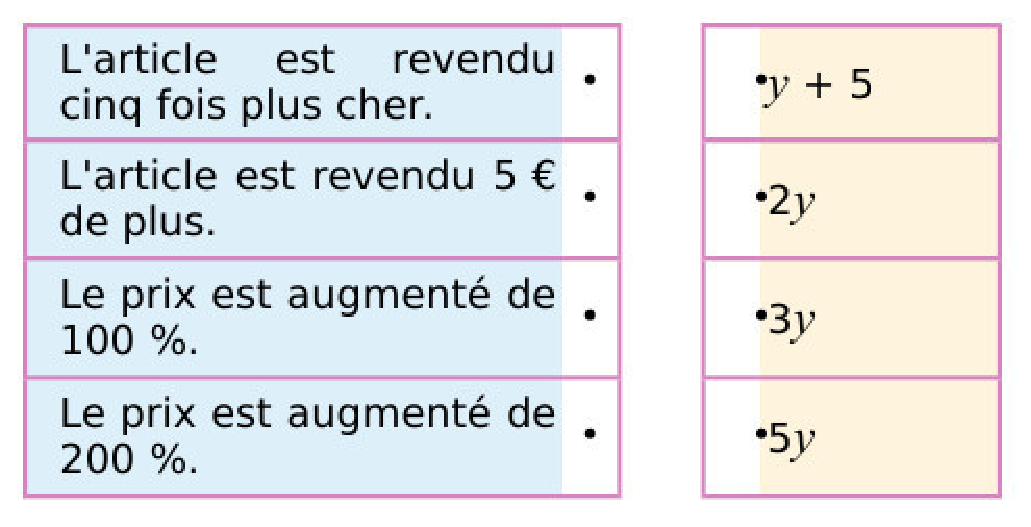
\includegraphics[width=.8\linewidth]{tableau2}
\end{center}
\end{exercice}

\begin{exercice}
Soient les deux programmes de calculs suivants :

Programme 1 :
\begin{itemize}
    \item Choisis un nombre ;
    \item Ajoute 6 à ce nombre ;
    \item Multiplie le résultat par -2 ;
    \item Ajoute le quadruple du nombre choisi au départ.
\end{itemize}

Programme 2 :
\begin{itemize}
    \item Choisis un nombre ;
    \item Soustrais 3 à ce nombre ;
    \item Multiplie le résultat par 4 ;
    \item Soustrais le double du nombre choisi au départ.
\end{itemize}

\begin{colenumerate}{1} 
\item Teste ces deux programmes de calculs pour $x = 2$ ; pour $x = -3$ et enfin pour $x = 4$.
\item\label{CLex42} Que remarques-tu ?
\item Si l'on note $x$ le nombre choisi au départ, écris une expression $A$ qui traduit le programme 1. 
\item De la même manière, écris une expression $B$ pour le programme 2.
\item Comment peux-tu expliquer la remarque faite à la question \ref{CLex42} ?
\end{colenumerate} 
\end{exercice}




 
\serie{Réduire}





\begin{exercice}
Réduis, si possible, les expressions suivantes :

\begin{colenumerate}{4} 
\item $x + x$
\item $x \times x$
\item $2x + x$
\item $3x + 2$
\item $2x \times x$
\item $x^2 + x$
\item $0 \times x$
\item $1 + 2x$
\item $0 + x$
\item $5x \times 6x$
\item $4 \times x \times 5$
\item $x \times x + x$
\end{colenumerate} 
\end{exercice}

\begin{exercice}
Réduis et ordonne, si possible, chacune des expressions suivantes :

\begin{colenumerate}{2} 
\item $12x -y + 2$
\item $7y + 12 -13y$
\item $10 -8d + 3$
\item $8 -x + x^2 + 5x$
\item $3t -12t + t^2 -7$
\item $a^2 + b -a + 3b $
\end{colenumerate} 
\end{exercice}

\begin{exercice}
Réduis les expressions suivantes :

\begin{colenumerate}{2} 
\item $\dfrac{3x}{2} + \dfrac{x}{4}$
\item $\dfrac{5x}{6}+\dfrac{x-4}{3}$
\item $3 + \dfrac{x-1}{5}$
\item $-5x - \dfrac{3x-2}{4} + 3$
\end{colenumerate}
\end{exercice}

\end{colonne*exercice}


%\exercicesappr
%\begin{colonne*exercice}
%\input{CalculLitteral/CalculLitteral_exos_approf}
%\end{colonne*exercice}

%\connaissances
%\input{CalculLitteral/CalculLitteral_qcm.tex}

%\TravauxPratiques
%\input{CalculLitteral/CalculLitteral_enGrp.tex}

%\recreation % avec R majuscule pour saut de page
%\input{CalculLitteral/CalculLitteral_finChap.tex}


